\chapter{聴覚と音声信号}
\section{\kadaida}\label{sec:\kadaida}
\purpose
\paragraph{音脈分凝とは}
例として,音列\ \fbox{C4\ G4\ C4\ G4\ C4\ G4\ \dots}\ をあげる.この音列を長く聴いた場合,テンポが遅いと音列は「旋律」として聞こえるが,テンポを早くするについれて\ \fbox{C4\ C4\ C4\ \dots} \ \fbox{G4\ G4\ G4\ \dots}と,音列が分離して聞こえる.
この現象を音脈分凝と呼ぶ.また,テンポを一定にした場合,2つの音程差(C4とG4は完全5度)が大きいほど,音脈分凝が生じやすい.\cite[p.182]{感覚知覚心理学}
\paragraph{実験}
今回の実験では,テンポを一定にした場合の,周波数による音脈分凝の生じ方について調査する.
音脈分凝が生じる波形を作成し,音脈分凝が生じる周波数組み合わせと,音脈分凝が生じにくい組み合わせを実験により発見する.
\method
サンプリング周波数を\(16\textrm{kHz}\),1音を\(0.2\)秒に設定し,音Aと音Bを連結させた音Cを10回繰り返す.
正弦波の行列を連結するために,\texttt{repmat}関数を用いる.実験する周波数の組み合わせを\tblref{tbl:音脈分凝_実験結果}に示す.周波数\(f_A\)と周波数\(f_B\)の差を\(f_D=\big|f_A-f_B\big|\)と定義する.
\scall\sref{src:04_01}
\result
聴音確認による結果を\tblref{tbl:音脈分凝_実験結果}に示す.
\begin{table}[h]
    \centering
    \caption{音脈分凝\ 実験結果}
    \label{tbl:音脈分凝_実験結果}
    \begin{tabularx}{\textwidth}{ccccR}
            & 周波数\(f_A\) & 周波数\(f_B\) & 周波数差\(f_D\) & \multicolumn{1}{c}{実験結果}                                    \\
        \hline
        実験1 & \(1000\)   & \(990\)    & \(10\)      & 音脈分凝は生じず,滑らかな音に聞こえた.                                        \\
        実験2 & \(1000\)   & \(800\)    & \(200\)     & 音脈分凝は生じず,別音の組み合わせによる旋律に聞こえた.                                \\
        実験3 & \(1000\)   & \(200\)    & \(800\)     & 音脈分凝が生じ,\(1000\textrm{Hz}\),\(200\textrm{Hz}\)の2音が分離して聞こえた. \\
        \hline
    \end{tabularx}
\end{table}
\consideration
結果より,周波数組み合わせの差\(f_D\)が大きいほど音脈分凝が生じやすいこと,\(f_D=10\)程度であれば音の切れ目すら聞こえないことが分かった.
今回の実験では,3つの組み合わせのみ実験したため,音脈分凝が生じる具体的な周波数差\(f_D\)は分からなかった.\par
音脈分凝の生じやすさは,個人の近くに左右されるので正確な実験方法,テンポによる音脈分凝の生じやすさについても,今後の課題として調査したい.
\section{\kadaidb}\label{sec:\kadaidb}
\purpose
\paragraph{連続聽効果とは}
ある一連の音を一部,短時間だけ削除し,雑音に置き換える.
ヒトは,「もとの音声の中に雑音が混入された」と知覚し,部分的な削除には気付かない.この現象を聴覚的補完,または連続聴効果と呼ぶ.\cite[p.182\ -\ p.183]{感覚知覚心理学}
\paragraph{実験}
連続聴効果が生じやすい刺激と,連続聴効果が生じにくい刺激を作成する.雑音や純音の周波数と,連続聴効果の関係について明らかにする.
\method
\paragraph{雑音の作成}
雑音を,白色雑音(ノイズA)と白色雑音からフィルタ処理により,周波数の\(1020\textrm{Hz}\)から\(1620\textrm{Hz}\)を除去した雑音(ノイズB)を作成する.
白色雑音は,振幅\(1\),サンプリング周波数\(16\texttt{kHz}\)で構成する.白色雑音は,周波数成分を均等に含むパワースペクトルが一定である,不規則な波である.(\ref{sec:\kadaiae}節)
ゆえに,乱数を\texttt{rand}関数を用いて生成し,白色雑音を作成する.
\texttt{rand}関数は,\(0\)から\(1\)までの実数を戻り値としているため,\texttt{rand}関数で\(-1\)から\(1\)までの実数を戻り値としたいときは,各要素から\(-0.5\)し,全データを\(2\)倍する.\par
周波数の\(1020\textrm{Hz}\)から\(1620\textrm{Hz}\)を除去するとき,\texttt{fft}の戻り値を考慮してフィルタを作成する.(\srcref{src:白色雑音の作成})
\figref{fig:ノイズAのFFT後}と\figref{fig:ノイズBのFFT後}を比較すると,ノイズBに周波数フィルタの適用が確認される.
フィルタを通した振幅スペクトルに対して,逆フーリエ変換することで音波を形成する.\par
\paragraph{純音の作成}純音の周波数は,純音A\(=400\textrm{Hz}\),純音B\(=1300\textrm{Hz}\)で作成する.
\paragraph{連続聴効果が生じる音刺激の作成}純音\(1\)秒,雑音\(0.1\)秒を4回繰り返す.実験する周波数の組み合わせを\tblref{tbl:連続聴効果}に示す.
\begin{lstlisting}[caption={白色雑音の作成},label={src:白色雑音の作成}]
white_noise = 2 * (rand(1,Fs) - 0.5); % 白色雑音の作成
B_fft = fftshift(fft(白色雑音)); % フーリエ変換
noise_filter = ones(1,Fs);
filter_rangeS = 1020; % カット始 周波数
filter_rangeG = 1620; % カット終 周波数
noise_filter((Fs/2)-filter_rangeG : (Fs/2)-filter_rangeS) = 0; % フィルタの作成
noise_filter((Fs/2)+filter_rangeS : (Fs/2)+filter_rangeG) = 0; % フィルタの作成
B_fft = noise_filter.* A_fft; % 各要素とフィルタの積を取る
noise_B = real(ifft(ifftshift(B_fft))); % 虚部を含むため,real関数を用いる
\end{lstlisting}
\begin{figure}[H]
    \centering
    \begin{minipage}{.45\textwidth}
        \centering
        \caption{ノイズAの\texttt{fft}後}
        \label{fig:ノイズAのFFT後}
        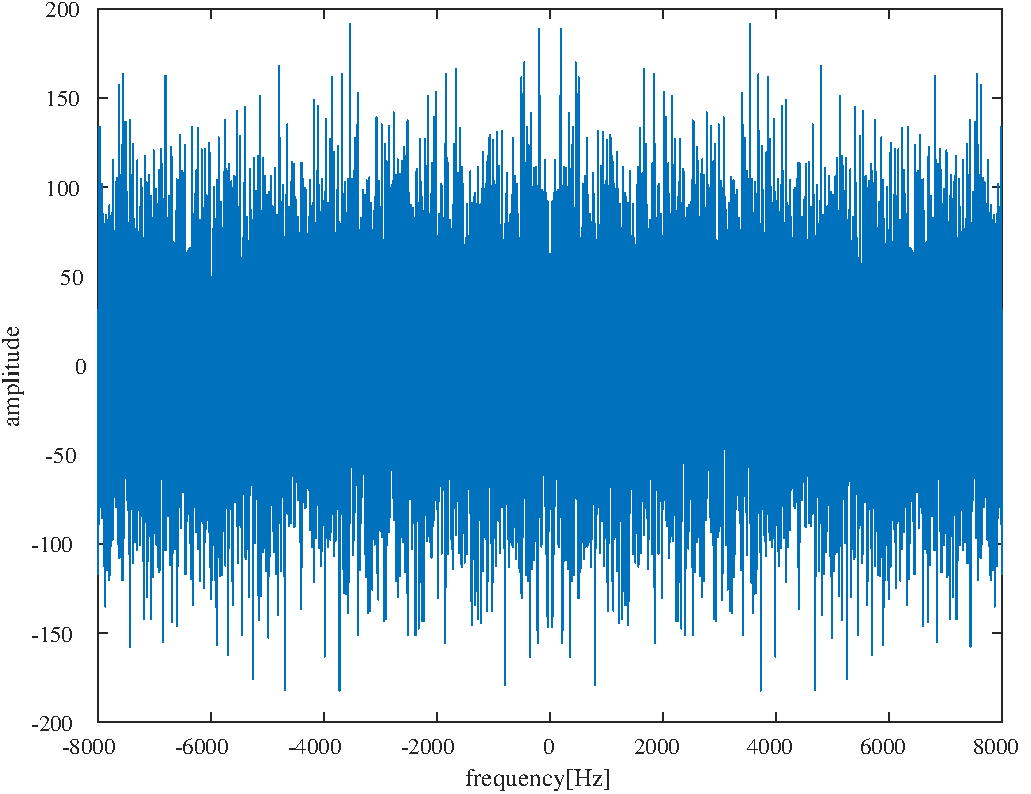
\includegraphics[keepaspectratio,width=\textwidth]{../../Figures/04_20_Afft.pdf}
    \end{minipage}
    \hspace{1em}
    \begin{minipage}{.45\textwidth}
        \centering
        \caption{ノイズBの\texttt{fft}後}
        \label{fig:ノイズBのFFT後}
        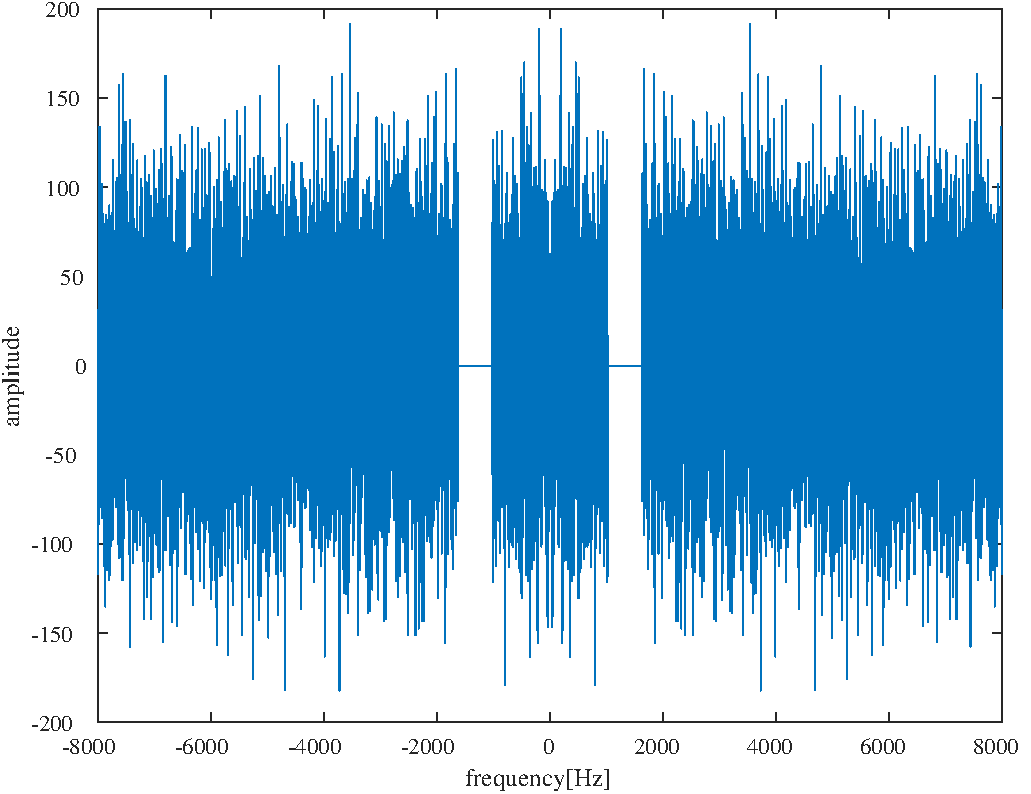
\includegraphics[keepaspectratio,width=\textwidth]{../../Figures/04_21_Bfft.pdf}
    \end{minipage}
\end{figure}
\result
実験結果を\tblref{tbl:連続聴効果}に示す.
\begin{table}[h]
    \caption{連続聴効果の実験組み合わせと結果}
    \label{tbl:連続聴効果}
    \begin{tabularx}{\textwidth}{cccR}
            & 純音  & 挿入するノイズ & \multicolumn{1}{c}{実験結果}  \\
        \hline
        実験1 & 純音A & ノイズA    & 雑音部で小さい純音が聞き取れた.          \\
        実験2 & 純音A & ノイズB    & 雑音部で小さい純音が聞き取れた.          \\
        実験3 & 純音B & ノイズA    & 雑音部で小さい純音が聞き取れた.          \\
        実験4 & 純音B & ノイズB    & 雑音部で純音は聞き取れず,純音が非連続に聞こえた. \\
        \hline
    \end{tabularx}
\end{table}
\consideration
実験結果より,純音の周波数がノイズの周波数に含まれていないとき,連続聴効果は生じなかった.
挿入されるノイズに純音の周波数が含まれているとき,雑音の周波数を基に,脳内で純音を補完していると考えられる.
ゆえに,純音の周波数をノイズから削除すると,連続聴効果が生じにくいと考えられる.\par
今回は純音に対する連続聴効果を実験したが,馴染み深い言語(日本語のフレーズ)に対して雑音を挿入すると,純音に比べて連続聴効果を知覚できるのではないだろうか.これは今後の課題として調査したい.